\section{Nuclei galattici attivi} \label{sec:nuclei-galattici-attivi}
La radiazione che riceviamo dalla galassie è principalmente dovuta alle stelle. Ma ciò non è vero per tutte le galassie, in particolare ce ne sono alcune in cui si è notato un nucleo centrale estremamente brillante la cui radiazione non è dovuta alle stelle. In altri casi si sono notati delle masse di gas uscenti dalla galassia; il caso più eclatante è quello della galassia Hercules A (in figura~\ref{fig:hercules-a}), in cui si può vedere come nella banda del visibile sia una galassia ellittica, ma quando osservata in banda radio vediamo due spettacolari getti di plasma.

\begin{figure}
    \centering
    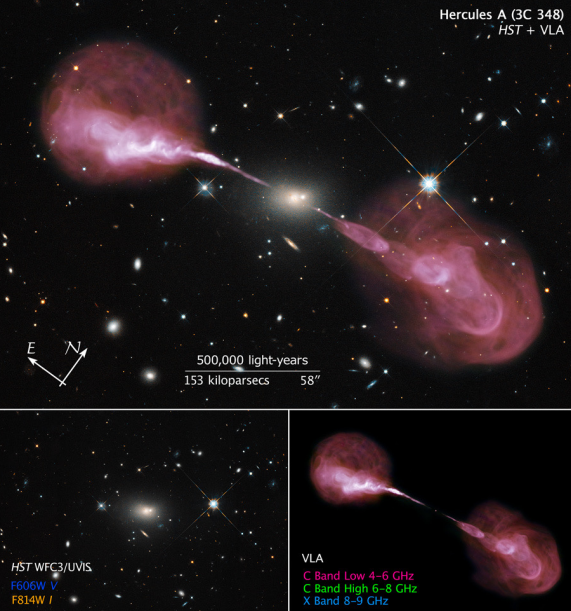
\includegraphics[width = 0.6\textwidth]{immagini/hercules-a.png}
    \caption{Galassia Hercules A (visibile e banda radio). \\ Da notare alcune stelle con la X di luce: sono stelle della NOSTRA galassia.}
    \label{fig:hercules-a}
\end{figure}

La presenza di un nucleo centrale estremamente brillante ma non stellare è tipico dei cosiddetti nuclei galattici attivi (AGN = Active Galactic Nuclei). Un AGN è definito come una regione compatta nel centro di una galassia che emette radiazione che non può essere attribuita a attività stellare ma è in gran parte dovuta a un fenomeno di accrescimento di gas di polvere su un buco nero centrale super massiccio (ossia con massa $> 10^6 \;\si{\solarmass}$). 

\subsection{Proprietà e tassonomia degli AGN}

Le più importanti caratteristiche osservative di una AGN sono:
\begin{itemize}
    \item una luminosità bolometrica molto alta (fino a $L_{bol} \sim 10^{48} \;\si{erg}/\si{s} \sim 3\cdot 10^4 L_{Milky Way}$).
    \item radiazione UV (non stellare), assieme a radiazione infrarossa e visibile.
    \item emissione di raggi X molto intensa.
    \item emissione non termica in un largo range di luminosità.
    \item spettro di emissione permesso con righe spettrali larghe.
    \item spettro di emissione permesso (e proibito) con righe spettrali strette. 
    \item getti relativistici emessi dal nucleo.
    \item variabilità temporale (da minuti ad anni) della continuità delle linee di emissione.
\end{itemize}
Non tutti gli AGN però mostrano queste caratteristiche: è stata sviluppata una tassonomia complicatissima di classi e sottoclassi di AGN sulla base della presenza o assenza di alcune quantità osservate ("AGN zoo").

Una tassonomia semplificata degli AGN può essere fatta in due modi:
\begin{itemize}
    \item Divisione in base allo spettro: indichiamo con AGN di Tipo 1 quelli che hanno linee di emissione sia larghe che strette e con AGN di Tipo 2 quelli che hanno solo linee di emissione strette.
    \item Divisione a seconda dell'emissione in banda radio: 
    \begin{equation*}
        \frac{F_{radio}}{F_{ott}} << 1 \quad \rightarrow \quad \text{RADIO QUIET (Quasars, QSOs, Sayfert galaxies)}
    \end{equation*}
    \begin{equation*}
        \frac{F_{radio}}{F_{ott}} >> 1 \quad \rightarrow \quad \text{RADIO LOUD (Quasars, QSOs, radio galaxies, BL Lac)}
    \end{equation*}
\end{itemize}

\subsection{Tipi di AGN}
\subsubsection{Quasars e QSOs}
Indichiamo con \emph{quasar} (che sta per "quasi-stellar" radio source) un oggetto sorgente di onde radio a distaze cosmologiche, con morfologia puntiforme (quindi simile a una stella) nella banda ottica. 

Indichiamo con \emph{QSOs} (che sta per "quasi-stellar" object) una sorgente di radiazione a distanze cosmologiche che ha morfologia puntiforme (quindi simile a una stella) nella banda ottica, ma con emissione in banda radio nulla o molto debole.

Tutti questi oggetti godono di alcune caratteristiche principali osservate:
\begin{itemize}
    \item sono i più luminosi fra tutti gli AGN ($L_{bol} \sim 10^{45}-10^{48} \;\si{erg}/\si{s}$).
    \item spettro di emissione con larghe linee di emissione permette e strette linee di emissione proibite.
    \item linee spettrali spostate molto verso il rosso.
    \item spesso presentano un colore blu (eccesso di UV) a una temperatura fissa e pari a $T\sim 2.5\cdot 10^4 \;\si{K}$.
    \item 90\% dei quasar sono radio quiet, 10\% sono radio loud.
\end{itemize}

Uno di questi oggetti si chiama 3C 273: è il primo quasar che è stato scoperto e si chiama così perché è il 273esimo oggetto del "Third Cambridge Catalogue of Radio Sources". Di questo oggetto sono stati fatti numerosi studi, in particolare è stata determinata con accuratezza la sua posizione, è stata identificata la sua controparte ottica (ossia la galassia ellittica di cui è il centro) e è stato misurato il suo redshift dalle linee di emissione del visibile. 

\subsubsection{Galassie Seyfert}
Il nome viene dallo scopritore di queste galassie, che ha iniziato a osservarle nel 1943. Sono galassie a disco con alta brillanza superficiale nelle regioni del nucleo (come tutte le AGN) e mostrano righe di emissione molto intense alta luminosità bolometrica ma inferiore di quella dei quasar.
Sono il tipo di AGN più comune nell’universo locale e sono al 95\% radio quiet (emissione in banda radio ma non particolamente forte).

A loro volta sono suddivise in due classi: 
\begin{itemize}
    \item Seyfert 1: forte emissione continua del nucleo non termica, con linee di emissione molto strette ma con spettro molto ampio. Sono inoltre caratterizzate da un'emissione di raggi X intensa e variabile (ore - giorni).
    \item Seyfert 2: Meno luminose delle Seyfert 1, mostrano solo righe di emissione strette (quindi sono AGN di Tipo 2). In più l'emissione di raggi X è molto debole o non presente; il motivo (spiegato più avanti) è che questa radiazione è assorbita da materiale che si interpone tra la Seyfert e noi osservatori. 
\end{itemize}

\subsubsection{Galassie radio}
Come dice il nome sono state classificate in base alla emissione radio; sono galassie con forte emissione radio, la loro luminosità radio confrontabile con i quasar radio loud. Sono caratterizzati dal fatto che la loro galassia è direttamente osservabile (a differenza dei quasar, per i quali è difficile osservare la galassia ospite). Le galassie ospite sono soprattutto galassie ellittiche, ma qualche volta la galassia ospite mostra una morfologia complessa o disturbata, sintomo di una interazione in atto con un'altra galassia. Alcune galassie radio hanno righe di emissione sia larghe che strette, altre hanno solo righe strette 

Anche qui sono presenti due sottoclassi (confronto in figura~\ref{fig:galassie-radio}):
\begin{itemize}
    \item FR I: sono meno lunminose nella banda radio, hanno un continuo ottico e delle righe di emissione più deboli delle FR II. Hanno una discreta varietà di morfologie radio e mostrano dei getti radio molto estesi che partono dal nucleo e si allungano fino a scale dell’ordine dei $\si{Mpc}$; questi getti sono però meno collimati di quelli delle FR II.  
    \item FR II: hanno dei getti radio altamente estesi e collimati e hanno lobi radio che mostrano anche degli hot spots (regioni piccole rispetto al logo dove la brillanza superficiale radio è estremamente elevata). 
\end{itemize}

\begin{figure}
    \centering
    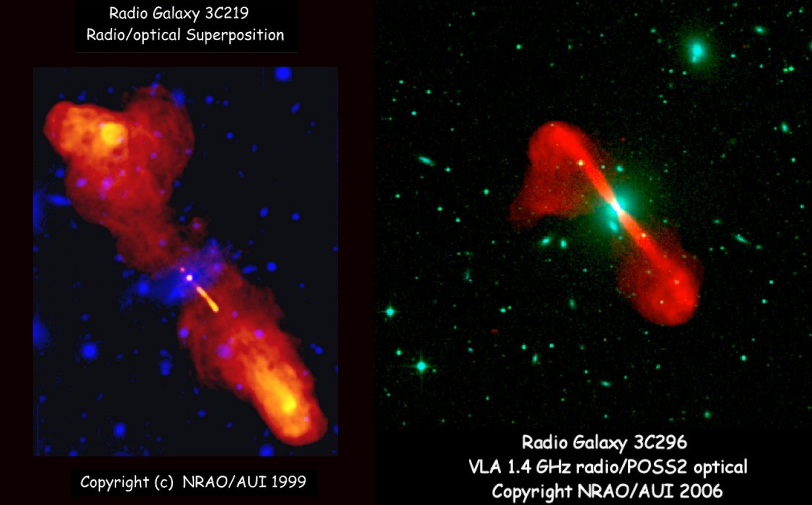
\includegraphics[width = 0.8 \textwidth]{immagini/galassie-radio.png}
    \caption{Confronto fra FR I (destra) e FR II (sinstra): le FR II mostrano raggi più collimati e gli hot spots, assenti invece nelle FR I.}
    \label{fig:galassie-radio}
\end{figure}

\subsubsection{BL Lacertae} 
Il termine BL è usato perchè identifica una classe di stelle variabili e il primo AGN di questo tipo è stato osservato nella costellazione della Lacerta: da lì in poi il nome è questo, solitamente abbreviato in BL Lac. 

Sono contraddistinte da una morfologia star-like (quindi puntiformi), con una variabilità forte e molto rapida (tempi scala brevissimi, fino a circa 10 min); la variabilità dipende dalla lunghezza d’onda (si allunga a lunghezze d’onda più lunga, con i tempi scala che diventano ore ad alte energie, quindi in banda X, e addirittura settimane o mesi nel visibile). Sono molto luminose in banda radio e mostrano un continuo ottico privo di righe (solo di rado si osservano righe di emissione e assorbimento, molto deboli); in più sono molto luminose in gamma. I getti sono orientati a piccoli angoli rispetto alla linea di vista dell’osservatore (circa 20°): ciò significa che non vediamo tutto il getto (90 gradi) ma un getto compattato.

In più sono una sottoclasse delle blazars (sorgenti altamente energetiche, variabili e molto compatte associata a un buco nero supermassiccio situata al centro di una galassia ospitante; sono tra i più violenti fenomeni nell'universo e sono un importante argomento di studio dell'astronomia extragalattica).

\subsection{Anatomia degli AGN}
Abbiamo visto che i vari tipi di AGN hanno caratteristiche diverse. Ma quindi sono oggetti fisici diversi questi vari tipi di AGN? No, si pensa che tutti gli AGN siano in realtà lo stesso oggetto dal punto di vista fisico, cambia solamente la linea di vista con cui osserviamo l’oggetto; questa idea va sotto il nome di \emph{modello unificato degli AGNs}.

\begin{figure}
    \centering
    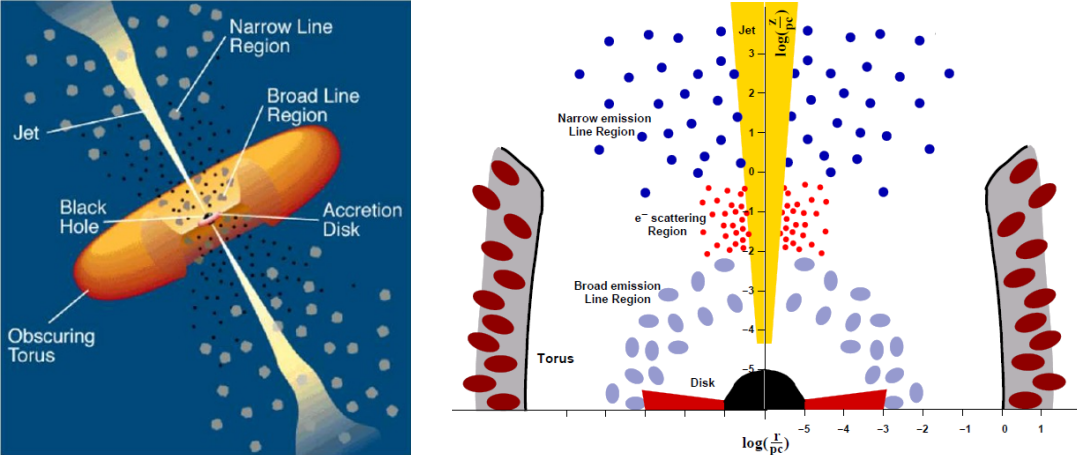
\includegraphics[width = \textwidth]{immagini/sezione-e-anatomia-agn.png}
    \caption{Anatomia degli AGN, con visione esterna e sezione mediale.}
    \label{fig:sezione-e-anatomia-agn}
\end{figure}

Prima di capire perché l’angolazione diversa dovrebbe portare a proprietà osservate diverse, vediamo l’anatomia di un AGN (fare riferimento alla figura~\ref{fig:sezione-e-anatomia-agn}):
\begin{itemize}
    \item Buco nero super massiccio: è il motore centrale dell'AGN (con massa $\sim 10^8 \;\si{\solarmass}$).
    \item Disco di accrescimento attorno al buco nero: è materiale caldo luminoso che sta spiraleggiando sul buco nero disponendosi su un disco molto piccolo (cade nel buco nero, $r \sim 10^{-3} \;\si{pc}$). In figura~\ref{fig:sezione-e-anatomia-agn} viene rappresentato dalle sezioni rosse intorno al buco nero. 
    \item Toro di polvere (gas denso e freddo + polvere): il toro circonda il nucleo ed è confinato dalla pressione esercitata dal gas più interno ($d \sim 1 \;\si{pc}$). In figura~\ref{fig:sezione-e-anatomia-agn} viene rappresentato dalle sezioni grige a sinistra e destra.
    \item Regione delle righe larghe (broad line region): regione vicina al disco di accrescimento del buco nero ($d \leq 0.01 \;\si{pc}$). Sono nubi di gas altamente ionizzato che si trovano nelle vicinanze del disco di accrescimento e si muovono con altissime velocità con moti turbolenti. In figura~\ref{fig:sezione-e-anatomia-agn} sono rappresentate dagli ovali azzurri chiari intorno al buco nero. 
    \item Regione delle righe strette (narrow line region): sono nubi di gas lontane ($d \sim 100 \;\si{pc}$) che si muovono a velocità inferiori di quelle nella broad line region. In figura~\ref{fig:sezione-e-anatomia-agn} sono rappresentate dai pallini azzurri lontani. 
    \item Getti: getti costituiti da particelle relativistiche cariche che partono dal nucleo e vanno verso l’esterno.
\end{itemize}

\begin{figure}
    \centering
    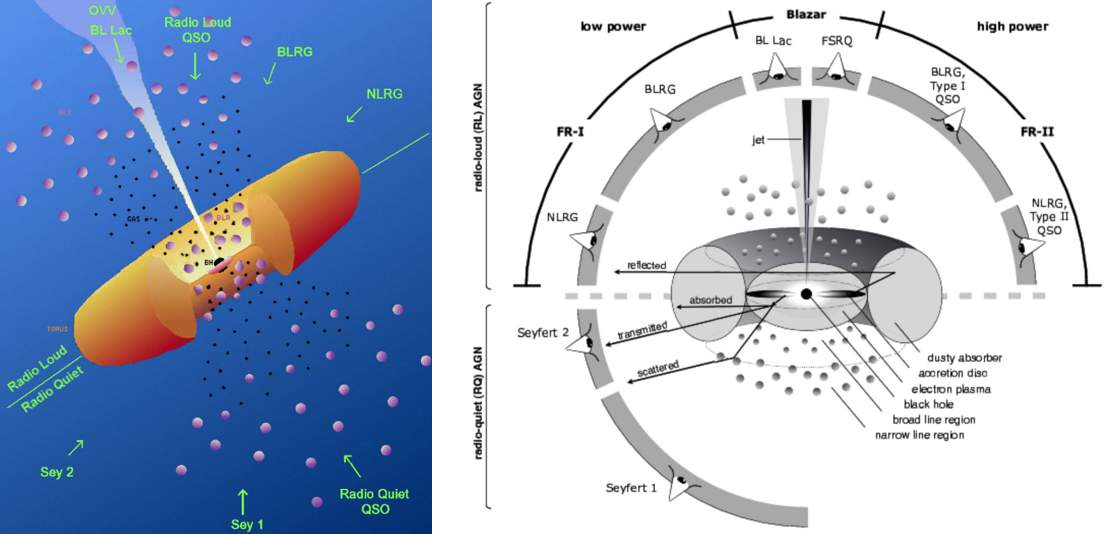
\includegraphics[width = \textwidth]{immagini/modello-unificazione-agn.png}
    \caption{Modello di unificazione degli AGN.}
    \label{fig:modello-unificazione-agn}
\end{figure}

In figura~\ref{fig:modello-unificazione-agn} possiamo vedere il modello di unificazione degli AGN: l'oggetto che osserviamo è sempre lo stesso, ma da linee di vista diverse quindi ci appaiono caratteristiche diverse. La cosa più interessante da notare è come lo spazio sia diviso in due zone, la prima radio loud (dove viene emesso il getto) e l'altra radio quiet (dove è emesso un contro-getto); per questo motivo gli AGN sono classificati in base alla radiazione radio emessa, proprio per distinguere da che parte stiamo osservando quest'oggetto. 

\subsection{Origine fisica dell'energia degli AGN}
L'energia degli AGN è principalmente di tipo gravitazionale, dovuta all'accelerazione di materia in un oggetto compatto e molto massivo (ossia il buco nero). L'energia irradiata per unità di tempo (ossia la luminosità) è data dall'espressione:
\begin{equation}
    \label{eq:luminosità-agn}
    L = G \frac{M\dot{M}_{acc}}{R}=\eta \dot{M}_{acc} \cdot c^2
\end{equation}
in cui $L$ è la luminosità di accrescimento e $\dot{M}_{acc}$ è la velocità di accrescimento di massa (può essere pensata come energia al secondo); $\eta$ è l'efficienza di conversione di energia gravitazionale in radiazione e ci ricorda che non tutta la massa accresciuta si trasforma in energia, ma soltanto una frazione (circa il 10\%). È sufficiente un tasso di accrescimento di materia piccolo (per esempio pari a $\sim 2 \;\si{\solarmass}/\si{yr}$) per spiegare le luminosità tipiche dei quasar. 

Questa espressione della luminosità di accrescimento ci permette di fare una prima stima grossolana della massa del buco nero. Come già ricordato non tutta l’energia gravitazionale viene convertita in luminosità, ma solo una frazione $\eta$; il resto va a finire in massa realmente accresciuta dal buco nero. Quindi abbiamo che (assumendo che $\eta$ sia costante e indipendente dal tempo):

\begin{equation*}
    \dot{M}_{BH} = (1-\eta) \dot{M}_{acc} \quad \rightarrow \quad \dot{M}_{acc} = \frac{1}{1 - \eta} \dot{M}_{BH}
    \quad \rightarrow \quad M_{acc} = \frac{1}{1 - \eta} M_{BH}
\end{equation*}

Allora l'energia irradiata da un AGN è data da:
\begin{equation*}
    E = L \cdot \tau =  M_{acc} \eta c^2 = \frac{\eta}{1 - \eta} M_{BH} c^2 \quad \rightarrow \quad M_{BH} = \frac{1-\eta}{\eta} \frac{L\tau}{c^2}
\end{equation*}

Assumendo $\eta = 0.1$, $\tau \sim 10^7/10^9 \;\si{yrs}$, $L \sim 10^{46} \;\si{erg}/\si{s}$ otteniamo una massa del buco nero$M_{BH} \sim 10^7/10^9 \;\si{\solarmass}$, il che lo rende quindi un buco nero supermassiccio; vediamo perchè possiamo giungere a questi dati e a questa conclusione.

\subsubsection{Luminosità di Eddington}
Dall'equazione~\refeq{eq:luminosità-agn} vediamo che la luminosità non può crescere a piacere ma è presente un limite superiore. Questo è dovuto ad una serie di step del processo:
\begin{itemize}
    \item La forza gravitazionale agisce principalmente sui protoni (perchè hanno massa molto maggiore degli elettroni), attrendoli verso il buco nero centrale.
    \item Questo produce una pressione di radiazione che invece agisce principalmente sugli elettroni, avendo questi una sezione trasversale più larga ($\propto (m_p/m_e)^2$).
    \item La pressione di radiazione separa le cariche e quindi si genera un campo elettrico che si oppone a gravità e pressione di radiazione rallentando l'accelerazione elettronica.
    \item Dopo che la luminosità irradiata da un certo corpo diminuisce, ovvero il campo elettrico risulta più forte della pressione verso l'esterno, allora il precedente meccanismo ricomincia (ossia la luminosità torna ad aumentare perchè riprende l'accrescimento del buco nero).
\end{itemize}
Sono tutti processi periodici, quindi la luminosità aumenta per poi diminuire e poi aumentare nuovamente. Il limite superiore raggiunto dalla luminosità prende il nome di \emph{luminosità di Eddington} ($L_{Edd}$). QUanto vale questo limite superiore per un AGN? Facciamo l'assunzione di un accrescimento sferico (anche se è un’approssimazione rozza perché avevamo visto che l’accrescimento avveniva su disco) e supponiamo ci sia una caduta radiale di idrogeno ionizzato verso il buco nero (tanto l'idrogeno è materiale più presente nell universo). La pressione di radiazione è data dal flusso radiativo diviso la velocità della luce, quindi possiamo calcolare la forza che agisce sul singolo elettrone (ossia la forza che allontana il singolo elettrone dal buco nero) come ($\sigma_T = 6.65 \cdot 10^{-25} \;\si{cm^{-2}}$ è la sezione trasversale di Thomson):
\begin{equation*}
    F_{rad} = \frac{L\sigma_T}{4\pi R^2 c}
\end{equation*}

D’altra parte possiamo calcolare la forza gravitazionale sul protone (consideriamo solo il protone perché la sua massa è molto più grande di quella dell'elettrone):
\begin{equation*}
    F_{grav} = G\frac{(m_p+m_e)M}{R^2} \simeq G\frac{m_pM}{R^2}
\end{equation*}

Se la forza sull’elettrone è maggiore della forza sui protoni, si genera un campo elettrico che si oppone all’accrescimento e se si ferma l’accrescimento la luminosità cala. Quindi abbiamo luminosità massima subito prima che ciò avvenga, ossia quando le due forze sono uguali (perché se $F_{rad} > F_{grav}$ diminuisce la luminosità). Uguagliando le due espressioni otteniamo la luminosità massima:
\begin{equation*}
    \frac{L\sigma_T}{4\pi R^2 c} =  G\frac{m_pM}{R^2} \quad \rightarrow \quad L = \frac{4\pi G c}{\sigma_T}m_pM = 1.26\cdot 10^38 \left(\frac{\textup{M}}{\si{\solarmass}}\right)\;\si{erg}/\si{s}
\end{equation*}

Ci sono anche dei casi in cui la luminosità di Eddington è ecceduta, semplicemente si spiega col fatto che alcune assunzioni fatte (come quella di accrescimento sferico) non sono rispettate. Se prendiamo quanto trovato come un'ordine di grandezza e utilizziamo il limite di Eddington è possibile trovare un limite inferiore per la massa; infatti la luminosità tipica di (per esempio) un QSO è $L\sim 10^{46} \;\si{erg}/\si{s}$, che però dev'essere minore della luminosità di Eddington:
\begin{equation*}
    L \leq 1.26\cdot 10^38 \left(\frac{\textup{M}}{\si{\solarmass}}\right)\;\si{erg}/\si{s} \quad \rightarrow \quad M \geq 10^8 \;\si{\solarmass}
\end{equation*}
Come ci aspettavamo otteniamo un oggetto molto massivo. 

\subsubsection{Compattezza del buco nero}

\begin{figure}
    \centering
    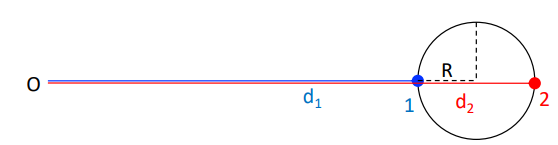
\includegraphics[width = 0.7 \textwidth]{immagini/compattezza-agn.png}
    \caption{Schema della compattezza degli AGN.}
    \label{fig:compattezza-agn}
\end{figure}

In un AGN le righe di emissione diventano più o meno intense nel tempo mostrando variazioni di luminosità anche molto rapide nel tempo; perché la variabilità degli AGN è una prova che sono compatti? Consideriamo una sfera di raggio R che diventa all’improvviso più brillante (rappresentata in figura~\ref{fig:compattezza-agn}). La radiazione viene emessa da tutta la sfera ma la radiazione emessa nel punto 1 impiega meno tempo di quella emessa nel punto 2 per arrivare all’osservatore. Questo fa si che l’osservatore vede un aumento di luminosità (radiazione da 1) che è diluito nel tempo (perchè la radiazione da 2 arriva dopo) su un tempo scala $\Delta t$ pari a $\Delta d/c = 2R/c$. Supponendo un tempo di variabilità di 1 ora si ha che il diametro della sorgente è dell’ordine di 7.2 AU. Quindi abbiamo un oggetto molto massiccio e molto compatto $\rightarrow$ super massive black hole!!!

\subsection{Distribuzione spettrale di energia (SED) negli AGN}

\begin{figure}
    \centering
    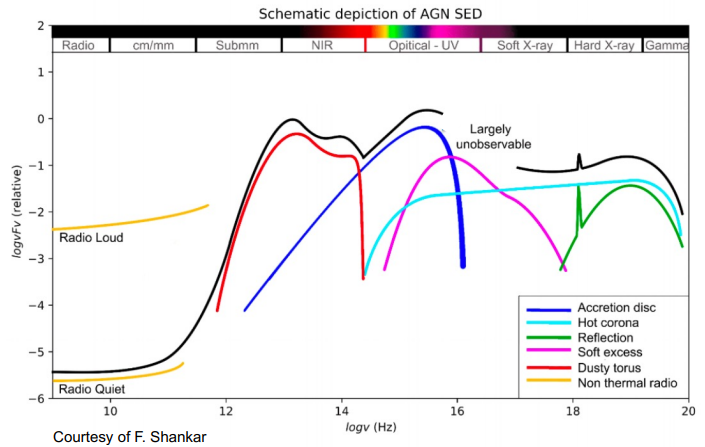
\includegraphics[width = 0.8 \textwidth]{immagini/sed-agn.png}
    \caption{Rappresentazione schematica della SED degli AGN.}
    \label{fig:sed-agn}
\end{figure}
In figura~\ref{fig:sed-agn} possiamo vedere la tipica SED degli AGN alle varie lunghezze d’onda, in cui sono anche evidenziate le principali sorgenti di radiazioni alle varie lunghezze d'onda. Dall’infrarosso fino ai gamma le SED degli AGN sono quasi piatte, ma vediamo cosa succede invece nelle altre regioni.

\subsubsection{Banda ottica}
La linea in blu in figura~\ref{fig:sed-agn} è in banda ottica e proviene principalmente dal disco di accrescimento. Come avviene l'emissione dal disco di accrescimento? Il gas nel disco cade verso il buco nero, perdendo energia potenziale; avendo però momento angolare non cade direttamente nel buco nero ma ci spiraleggia attorno. Dal trasferimento di momento angolare e dall'attrito con il resto del gas, il gas si arrangia nella forma di un disco orientato perpendicolarmente alla direzione del momento angolare. La rotazione del disco è approssimativamente kepleriana (rotazione differenziale, quindi la velocità dipende dal raggio) con il gas che si scalda a causa dell'attrito dinamico. (assunto sempre molto minore della forza gravitazionale). Lo stesso attrito causa un rallentamento delle particelle del gas, causando uno spiraleggiamento verso l'interno, convertendo energia potenziale in cinetica e poi in calore (quindi gli strati più interni sono decisamente più caldi). Possiamo notare che un corpo come questo è simile ad un corpo nero multicolore (anche in quel caso a seconda della temperatura abbiamo una radiazione diversa): quindi ciascun anello emette per corpo nero e noi possiamo pensarlo come un insieme di anelli concentrici. L'emissione che a questo punto noi osserviamo è quella da tutto il disco che è la composizione di molte emissioni di corpo nero (come si vede in figura~\ref{fig:emissione-del-disco-di-accrescimento}) e questo spiega la curva blu del grafico iniziale.

\begin{figure}
    \centering
    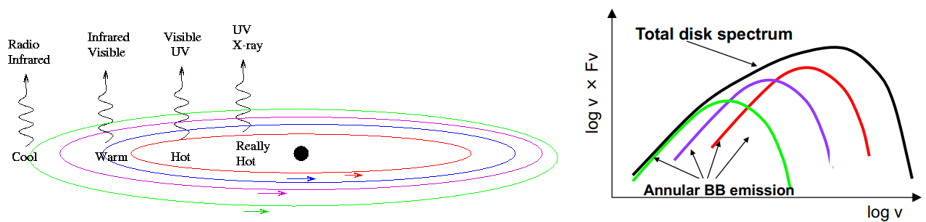
\includegraphics[width = \textwidth]{immagini/emissione-del-disco-di-accrescimento.png}
    \caption{Emissione del disco di accrescimento.}
    \label{fig:emissione-del-disco-di-accrescimento}
\end{figure}

\subsubsection{Banda IR}
In infrarosso abbiamo la linea rossa in figura~\ref{fig:sed-agn}: questa linea è la linea di emissione dal toro, perché il toro è composto in gran parte da gas freddo e quindi emette in banda infrarossa. 

 \subsubsection{Banda X}
L'emissione in banda X corrisponde alla riga azzurrina in figura~\ref{fig:sed-agn} ed è dovuta principalmente allo scattering di elettroni relativistici dalla “corona calda” dell'AGN. Si verifica infatti uno scattering di elettroni contro fotoni termici del disco di accrescimento e questo processo prende il nome di \emph{Effetto Compton inverso} (accenneremo alla fine del corso, ma in pratica il fotone acquista energia perché è meno energetico e l'elettrone perde energia). La "hot corona" è un’altra componente negli AGN ed è gas caldo attorno al buco nero, disposto ai poli del buco nero non occupati dal disco di accrescimento; si ritiene sia la maggior emettritrice in banda X ma non si sa come sia fatta la corona. L’idea è che sia plasma a bassa densità e molto caldo ma la geometria è ancora molto discussa (varie ipotesi che però non sono ancora state verificate).

\subsubsection{Banda radio}
Le emissioni in banda radio sono presenti sono in alcuni AGN (quelli radio loud) e sono principalmente dovute all'emissione radio a sincrotrone causata dagli "hot spot" e dai campi magnetici dovuti ai getti provenienti dal buco nero.
 
\subsection{AGN oscurati}
Abbiamo motivo di credere che ancora non abbiamo osservato tutti i tipi di AGN. Infatti un AGN può essere oscurato dal toro che assorbendo l'emissione X non permette di osservare l'oggetto; quindi a seconda delle linee di vista la parte dell'emissione X della SED può essere molto modificata (si dice assorbita), perché cambia la densità della colonna di gas interposta (che indichiamo con $N_H$). In particolare in base a questa grandezza possiamo dividere gli AGN oscurati in 3 categorie:
\begin{itemize}
    \item AGN non assorbiti: $\log N_H < 21$.
    \item AGN Compton-sottili: $21 < \log N_H < 24$.
    \item AGN Compton-spessi: Mildly ($\log N_H = 24/25$), Heavily ($\log N_H > 25$).
\end{itemize}
Il miglior modo per osservare questi oggetti è in infrarosso. 

Perché sappiamo che esistono questi oggetti anche se non possiamo osservarli? Perchè la loro esistenza è predetta dal modello unificato per spiegare il cosiddetto "X-Ray Background" (figura~\ref{fig:xrb-agn}). Infatti la distribuzione di emissioni in banda X è descritta dalla linea rosa in figura che fitta i dati sperimentali: possiamo vedere che per $E \leq 2-3 \;\si{keV}$ abbiamo quasi il 100\% dello spettro risolto, mentre per $E > 10 \;\si{keV}$ il contributo delle sorgenti risolte cala al di sotto del 50\%. Proprio il contributo mancante viene spiegato dagli AGN oscurati che non riusciamo ad osservare in banda X.

\begin{figure}
    \centering
    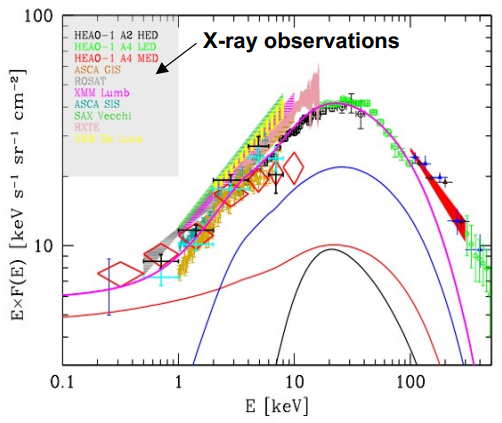
\includegraphics[width = 0.7\textwidth]{immagini/xrb-agn.png}
    \caption{"X-Ray Background": la linea rossa indica gli AGN non oscurati, quella blu i Compton Thin e quella nera i Compton Thick.}
    \label{fig:xrb-agn}
\end{figure}

\subsection{Linee spettrali}
Abbiamo visto che le linee di emissione osservate possono essere strette (Narrow Line Region, NLR) oppure larghe (Broad Line Region, BLR). 

Le prime sono dovute a nubi di gas con temperature $T \sim 10^2/10^3 \;\si{K}$ e una densità relativamente bassa $\rho \sim 10^3/10^4 \;\si{cm^{-3}}$ per permettere linee proibite. La NLR è più esterna rispetto al toro e viene osservata sia negli AGN di Tipo 1 sia in quelli di Tipo 2. 

Le seconde invece sono generate in nubi molto più calde e più dense ($T\sim 10^4 \;\si{K}$, $\rho \sim 10^{10}/10^{11} \;\si{cm^{-3}}$), con molte più linee proibite. Le BLR sono molto vicine al buco nero e muovendosi ad alte velocità ($v \sim 10^3/10^4 \;\si{km}/\si{s}$) abbiamo che le linee possono allargarsi a causa dell'effetto Doppler. Infine, proprio per la loro vicinanza al buco nero, le BLR possono essere oscurate dal toro e infatti le osserviamo solo negli AGN di Tipo 1.

Le BLR costituiscono un'ulteriore prova della presenza di un buco nero supermassiccio; infatti se assumiamo che queste regioni di gas siano confinate a causa della forza gravitazionale, dal teorema del viriale possiamo scrivere che:
\begin{equation*}
    v^2 = \frac{GM}{R} \quad \rightarrow \quad M = \frac{R}{G} v^2
\end{equation*}
Assumendo $R_{BLR}\sim 1 \;\si{pc}$ e $v \sim 5000 \;\si{km}/\si{s}$ otteniamo che $M_{BH} \sim 5 \cdot 10^9 \;\si{\solarmass}$, che è la massa caratteristica proprio di un buco nero supermassiccio.

\subsection{Co-evoluzione galassie e AGN} \label{co-evoluzione-galassie-agn}
Ci sono una serie di fatti che fanno supporre che gli AGN e le galassie che li ospitano evolvano insieme e l'evoluzione di uno causi delle modifiche nell'altro. Analizziamo questi fatti:
\begin{itemize}
    \item Tutte le galassie massive mostrano prove di un buco nero suermassiccio al centro, ma solo una piccola percentuale mostra la presenza di un AGN. Questo può essere spiegato da un "duty cicle": l'accrescimento di massa sul buco nero scalda i gas circostanti, ostacolando così ulteriore accrescimento. Quindi l'attività dell'AGN è auto-regolata e l'AGN è attivo solo per una minima frazione del tempo di vita della galassia ($\sim 10^{-3}/10^{-4}$).
    \item C'è una stretta correlazione fra la massa della galassia o la sua dispersione di velocità e la massa del buco nero supermassiccio (nonostante la differenza di quasi 9 ordini di grandezza fra le due scale!), quindi come se la grandezza del buco nero centrale implichi direttamente una massa della galassia e una sua dispersione delle velocità.
    \item Il tasso di formazione stellare e la crescita cosmica del buco nero (attività AGN) mostrano una dipendenza molto simile rispetto al tempo cosmico.
\end{itemize}

Tutti questi fatti indicano che ci deve essere una co-evoluzione di galassie e AGN: i processi di evoluzione delle galassie incidono sul loro buco nero centrale e allo stesso modo i processi di evoluione del buco nero supermassiccio incidono sull'evoluzione della galassia.

Possiamo vedere un riassunto del possibile schema evolutivo in figura~\ref{fig:coevolution-galassie-agn}. Partendo da in alto a sinistra abbiamo dei merger fra galassie ricche di gas: questi danno luogo a galassie starbust, il buco nero cresce e da carburante ad attività AGN (tipo SF o QSO). Poi il meccanismo di feedback del buco nero espelle gas e quindi spegne i processi AGN e si torna a galassie normali ("dead quasars"). Poi il processo può riniziare con nuovi merger \dots

\begin{figure}
    \centering
    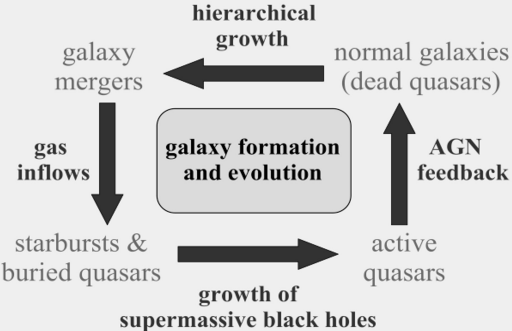
\includegraphics[width = 0.6 \textwidth]{immagini/coevolution-galassie-agn.png}
    \caption{Schema della co-evoluzione di galassie e AGN.}
    \label{fig:coevolution-galassie-agn}
\end{figure}

Ci sono ancora una serie di domande aperte però, per esempio, come si sono formati questi buchi neri supermassici?